% !TeX root = ../main.tex
% Add the above to each chapter to make compiling the PDF easier in some editors.

\chapter{Introduction}\label{chapter:introduction}
Use with pdfLaTeX and Biber.

\section{Section}
1. Experiments in GPU-based occlusion culling (Anagnostou, Interplay of Light) \cite{Anagnostou.2017}: \\
tldr CPU occlusion culling is very coarse as the CPU isn't great at rasterising. GPU can rasterise efficiently and supports hardware occlusion queries. Problem: "drawcall level" granularity, needs query and fence around every drawcall, thus can't handle instancing very well. Other problem: readback to CPU necessary, to avoid stalling use previous frame occlusion info for current frame. Thus popping likely for fast moving objects or camera. 
Other solution: render low res occlusion buffer on GPU, produce mip chain, determine screen-space size of each prop and compare vs appropriate mip-level of buffer. Still needs CPU readback though, unless... compute shader in modern API: "In this case I will be using a compute shader to perform the occlusion tests, producing a list of visible props that I will then be consuming on the GPU, avoiding the CPU roundtrip."\\

2. Why Frustum Culling Matters, and Why It's Not Important \cite{Barrett.2017}: \\
tldr disregardm, oversimplified explanation of frustum culling.\\

3. Overview on popular occlusion culling techniques \cite{gamesindustry.biz.2016}: \\
tldr temporal culling methods are prone to artifacting with fast object or camera movement, CPU culling "is the most efficient, forward-looking approach", then again the article is written by someone from Umbra3D, a CPU occlusion culling middleware. 
Still, precomputed visibility sets for weak devices are brought up, low res HI-Z depth buffer rasterised on the CPU with SIMD units for dynamic culling, see Intel's 2015/2016 occlusion culling article.\\

4. Frustum Culling \cite{Gerlits.2017}: \\
tldr code samples and brief performance numbers for bounding sphere, AABB, OBB based culling, SSE support, MT support, somewhat simple GPU culling. Sphere or AABB with SSE + MT support quite fast, 0.1-0.2ms for 100k objects on unspecified i5 quadcore.\\

5. Dual-Cone View Culling for Virtual Reality Applications \cite{Hale.2018}: \\
tldr not discernibly faster than frustum pyramid culling plus stencil mesh. Needs careful tuning for each HMD to avoid performing worse when a larger image is rendered and warped to view. With SIMD, more accurate cones etc may be more efficient.\\

6. Culling Techniques \cite{ITCS.Subramanian}: \\
tldr general explanation. Of interest maybe hierarchical bounding volumes for frustum culling. As the goal is a fast rendering of extreme number of objects, hierarchical ordering seems obviously necessary.\\

7. A Survey of Visibility for Walkthrough Applications \cite{CohenOr.2003}: \\
tldr .\\

8. Occlusion Culling Methods \cite{Hey.2001}: \\
tldr .\\

9. Math for Game Developers - Frustum Culling\cite{Rodriguez.2013}: \\
tldr as expected, brief mathematical explanation on how to compute whether a prop is inside the view frustum (based on position and prop radius).\\

10. Wie Sie einen Einstieg in das Frustum Culling finden \cite{VisCircleGmbH.}: \\
tldr D3D sample code for view frustum culling. Very brief, not very useful. But raises the questions how to compute (and store) bounding sphere radius for each prop, and how to compute and update frustum planes each frame (aka reconstruct from view + proj matrices or set up at start and then move all planes according to camera movement).\\

11. Superfrustum culling \cite{Whiting.2017}: \\
tldr instead of one frustum per eye, construct one superfrustum covering both. On paper means somewhat fewer objects are culled, but the reduced overhead still comes out on top. In their testing, shaved off ~1ms on lower end CPUs. Also monoscopic far-field for lower end devices and far draw distances: past a certain distance, stereo separation becomes very small, nigh indistinguishable, so it may be faster to render the far field monoscopic and then composit with the near-field stereo image. \\

12. OpenGL sample for shader-based occlusion culling \cite{Kubisch.2014}: \\
tldr shader-based batched occlusion culling system: leverages multi\char`_draw\char`_indirect and works well with setups where all geo is stored in one big buffer. \\

Thus, things up in the air: 
frustum culling, occlusion culling, detail culling, distance culling, hierarchical culling, cpu culling vs gpu culling, dual-view frustum culling vs superfrustum culling, stencil meshing, ...center-distance culling for foveated rendering, SIMD and MT optimization, ...

\subsection{Subsection}

See~\autoref{tab:sample}, \autoref{fig:sample-drawing}, \autoref{fig:sample-plot}, \autoref{fig:sample-listing}, \autoref{fig:tum}, \autoref{fig:tumslide}.

\begin{table}[htpb]
  \caption[Example table]{An example for a simple table.}\label{tab:sample}
  \centering
  \begin{tabular}{l l l l}
    \toprule
      A & B & C & D \\
    \midrule
      1 & 2 & 1 & 2 \\
      2 & 3 & 2 & 3 \\
    \bottomrule
  \end{tabular}
\end{table}

\begin{figure}[htpb]
  \centering
  % This should probably go into a file in figures/
  \begin{tikzpicture}[node distance=3cm]
    \node (R0) {$R_1$};
    \node (R1) [right of=R0] {$R_2$};
    \node (R2) [below of=R1] {$R_4$};
    \node (R3) [below of=R0] {$R_3$};
    \node (R4) [right of=R1] {$R_5$};

    \path[every node]
      (R0) edge (R1)
      (R0) edge (R3)
      (R3) edge (R2)
      (R2) edge (R1)
      (R1) edge (R4);
  \end{tikzpicture}
  \caption[Example drawing]{An example for a simple drawing.}\label{fig:sample-drawing}
\end{figure}

\begin{figure}[htpb]
  \centering

  \pgfplotstableset{col sep=&, row sep=\\}
  % This should probably go into a file in data/
  \pgfplotstableread{
    a & b    \\
    1 & 1000 \\
    2 & 1500 \\
    3 & 1600 \\
  }\exampleA
  \pgfplotstableread{
    a & b    \\
    1 & 1200 \\
    2 & 800 \\
    3 & 1400 \\
  }\exampleB
  % This should probably go into a file in figures/
  \begin{tikzpicture}
    \begin{axis}[
        ymin=0,
        legend style={legend pos=south east},
        grid,
        thick,
        ylabel=Y,
        xlabel=X
      ]
      \addplot table[x=a, y=b]{\exampleA};
      \addlegendentry{Example A};
      \addplot table[x=a, y=b]{\exampleB};
      \addlegendentry{Example B};
    \end{axis}
  \end{tikzpicture}
  \caption[Example plot]{An example for a simple plot.}\label{fig:sample-plot}
\end{figure}

\begin{figure}[htpb]
  \centering
  \begin{tabular}{c}
  \begin{lstlisting}[language=SQL]
    SELECT * FROM tbl WHERE tbl.str = "str"
  \end{lstlisting}
  \end{tabular}
  \caption[Example listing]{An example for a source code listing.}\label{fig:sample-listing}
\end{figure}

\begin{figure}[htpb]
  \centering
  \includegraphics[width=0.8\textwidth]{tum}
  \caption[Something else can be written here for listing this, otherwise the caption will be written!]{Includegraphics searches for the filename without extension first in logos, then in figures.} \label{fig:tum}
\end{figure}

\begin{figure}[htpb]
  \centering
  \includegraphics[width=0.8\textwidth]{figures/tum}
  \caption{For pictures with the same name, the direct folder needs to be chosen.} \label{fig:tumslide}
\end{figure}

\begin{figure}[!tbp]
  \centering
  \subfloat[TUM Logo][The logo.]{\includegraphics[height=0.2\textheight]{tum}\label{fig:tum1}}
  \hfill
  \subfloat[TUM Slide][The famous slide.]{\includegraphics[height=0.2\textheight]{figures/tum}\label{fig:tum2}}
  \caption{Two TUM pictures side by side.}
  \label{fig:sidebyside}
\end{figure}

This is how the glossary will be used.

\Glspl{ddye}, \gls{r0}, \gls{R0}, and \gls{kdeac}. Also, the \glspl{tum} has many \glspl{computer}, not only one \Gls{computer}. Subsequent acronym usage will only print the short version of \glspl{tuma} (take care of plural, if needed!), like here with \gls{tuma}, too. It can also be --> \glsdisp{tum}{hidden}\footnote{Example for a hidden TUM glossary entry.} <--.

\todo{Now it is your turn to write your thesis.

This will be a few tough weeks.}

\done{Nevertheless, celebrate it when it is done!}
